\section{Harness}
\label{sec:harness}

\begin{figure}[t]
    \centering
    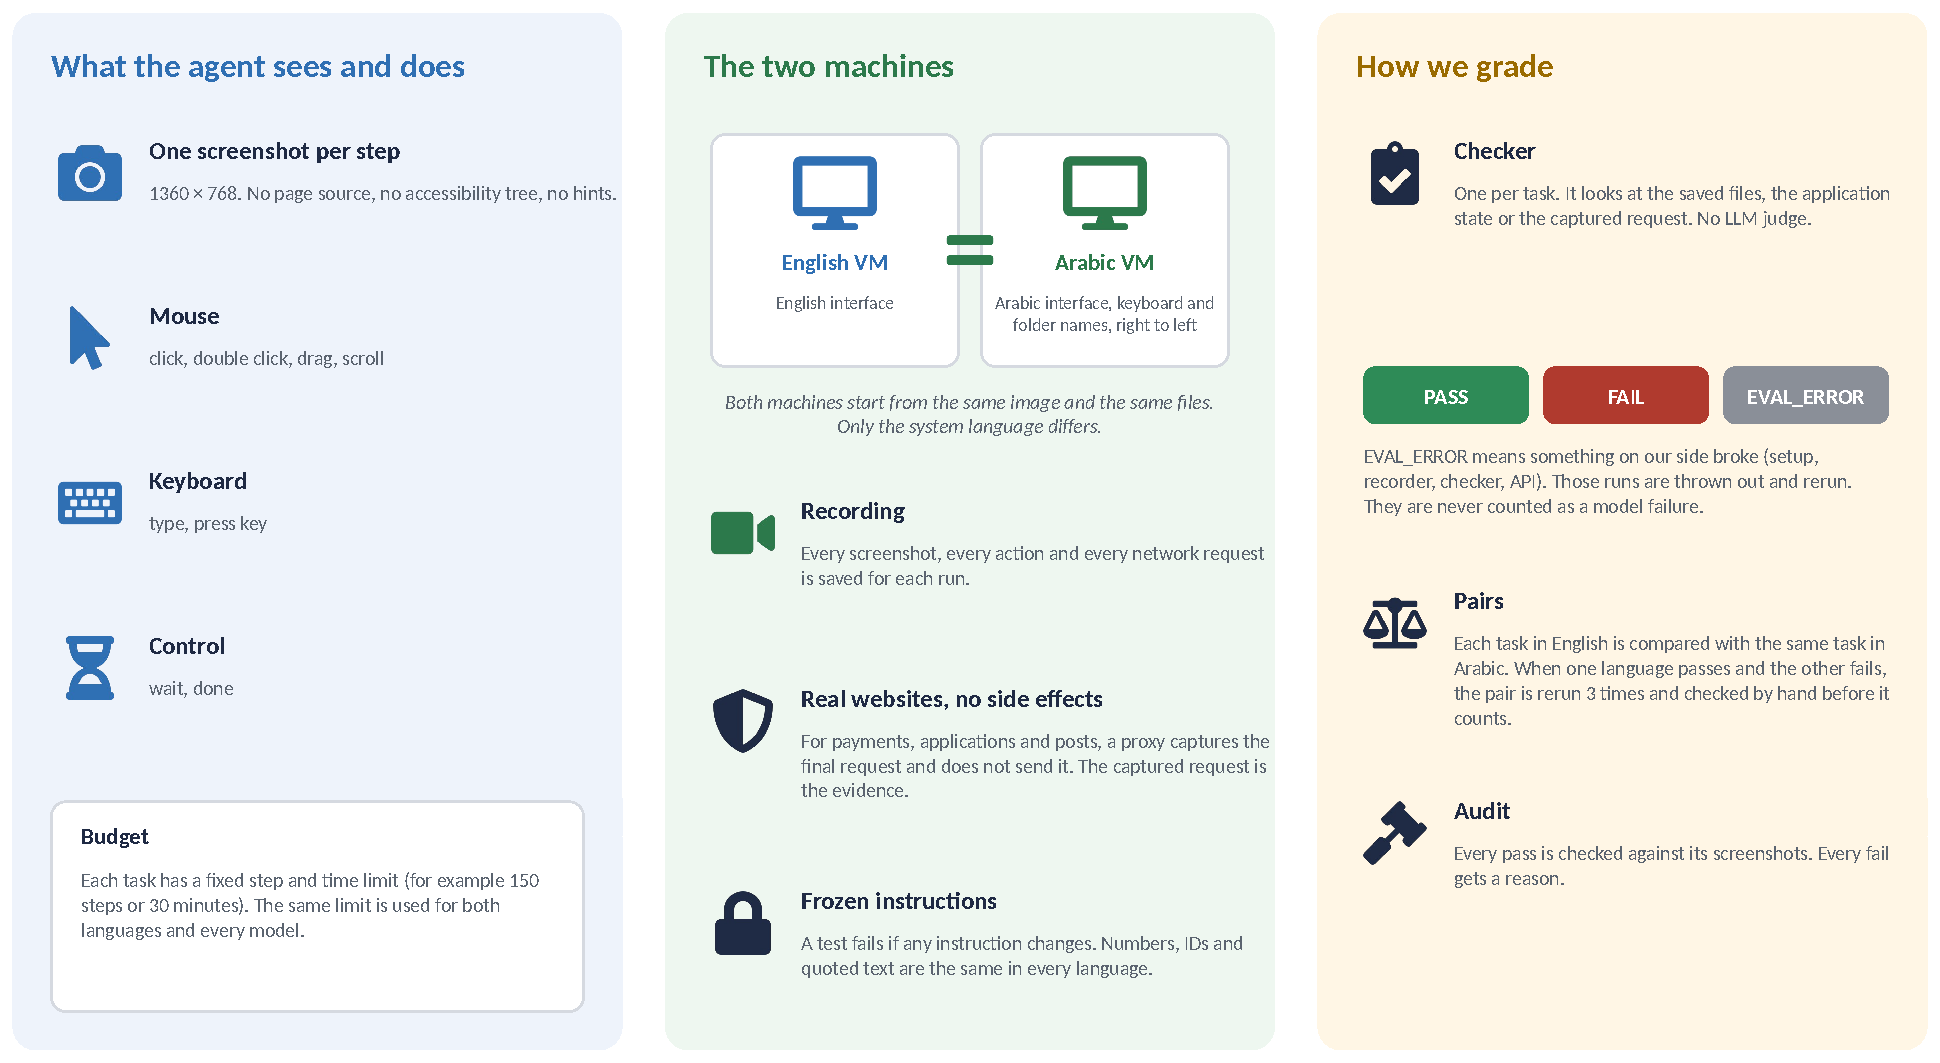
\includegraphics[width=\linewidth]{figures/fig2.pdf}
    \caption{The harness. Left: the agent receives one screenshot per step and
    acts through a small set of mouse and keyboard actions. Middle: the English
    and Arabic machines start from the same image and differ only in system
    language. Right: every run is recorded, consequential requests are captured
    and blocked, and a per-task checker returns pass, fail, or evaluation
    error.}
    \label{fig:harness}
\end{figure}

The harness runs one task on one machine with one model and produces a
recorded run and a verdict. It is deliberately simple. The agent gets what a
person gets, a screen and input devices, and nothing more.
Figure~\ref{fig:harness} gives the overview.

\subsection{What the agent sees and does}
\label{sec:agent}

\paragraph{Observation.}
At every step the agent receives one screenshot of the full desktop at
1360$\times$768 pixels. It receives nothing else: no page source, no
accessibility tree, no window titles, no file listings, and no hints. This is
a deliberate choice. Many agent benchmarks give the model an accessibility tree
or the DOM \citep{xie2024osworld, zhou2024webarena}. Those representations are
produced by the software, not seen by the user, and they hide exactly what we
want to measure: how the agent copes with an Arabic screen. Screenshots put
both languages on equal footing. The agent also receives the instruction, a
short identity sheet for the persona (name, address, email account; see
below), and the last three turns of its own history.

\paragraph{Actions.}
The agent has eight actions, listed in Table~\ref{tab:actions}. Each turn it
must choose exactly one. Coordinates are pixel positions on the screenshot,
counted from the top-left corner, and are never mirrored for Arabic: the agent
must find things where they actually are on a right-to-left screen. Actions
are executed on the machine through the standard X11 input-injection path
(\texttt{xdotool}), the same path a hardware keyboard and mouse use. The agent
has no shell. Requests for a shell or any other tool are refused and recorded.

\begin{table}[t]
\centering
\small
\begin{tabular}{ll}
\toprule
Action & Arguments \\
\midrule
click, double\_click & $x$, $y$ \\
drag & $x$, $y$, $x_{\text{to}}$, $y_{\text{to}}$ \\
scroll & $x$, $y$, $dy$ \\
type & text \\
key & one key or a chord (e.g.\ ctrl+s) \\
wait & seconds (1--10) \\
done & --- \\
\bottomrule
\end{tabular}
\caption{The action set. Every model gets the same eight actions. The
\texttt{done} action ends the run; it does not decide success.}
\label{tab:actions}
\end{table}

\paragraph{Model interface.}
Each model is called through its own native interface for structured actions
(function calling for GPT and Gemini, the computer-use tool for Claude), but
the action set, the screenshot, the instruction, the budget, and the history
window are identical. The system prompt tells the model it is operating a real
Linux desktop, that it has only the screenshot and ordinary mouse and keyboard
actions, and that \texttt{done} ends the episode but an independent checker
decides success. We record the interface used for each model because it is a
methods fact: a model with a native computer-use tool has a small structural
advantage in expressing actions, and we do not hide it.

\paragraph{Typing in Arabic.}
The Arabic machine has an Arabic keyboard layout. Typing Arabic text and
pressing keyboard shortcuts under that layout are two different problems for
the injection path, and both broke in early versions of the harness: shortcuts
such as ctrl+s resolved to the Arabic letter on the key and did nothing.
We fixed the injection so that shortcuts work under either layout without
switching the machine to a US layout, because forcing a US layout on the
Arabic machine would remove a real part of the Arabic experience.

\paragraph{Budget.}
Every task has a step limit and a wall-clock limit written into its package.
Borrowed web tasks use the limit adopted by ClawBench, thirty minutes, with a
step cap of 150; desktop and terminal tasks use limits sized to their length.
The limit is part of the task definition: it is identical for both language
arms and for every model, and it does not change during an experiment.

\subsection{The two machines}
\label{sec:machines}

Both arms run in KVM virtual machines built from the same Ubuntu 24.04 GNOME
image with the same applications: Chrome, LibreOffice, Thunderbird, GIMP, VLC,
VS Code, a text editor, a file manager, and a terminal. The image is built
twice, once with the English locale and once with the Arabic locale
(\texttt{ar\_QA}). The Arabic build has the Arabic language packs, Arabic fonts,
an Arabic keyboard layout, Arabic names for the standard folders, and a
right-to-left desktop. Its Chrome is set up the way an Arab user's Chrome is:
Arabic is the preferred language, and pages served only in English are
machine-translated by the browser. This last choice is important. Most
websites in our tasks do not ship an Arabic version, so what an Arab user
actually sees is Chrome's translation of the English page. We measure that,
because it is the real experience; we also record, for every web task, whether
the site served native Arabic or a browser translation, and report results by
that split.

Every run gets a fresh machine. A run starts by cloning a thin overlay from the
locale's base image, booting it, applying the task's setup, and waiting until
the desktop is ready. When the run ends the overlay is destroyed. Nothing
carries over between runs, and the two arms of a pair start from byte-identical
disk images apart from locale.

\paragraph{Persona and accounts.}
Web tasks that need an identity use one fictional persona, a Qatari resident
with a fixed name, address, and date of birth, presented in English on the
English machine and in Arabic on the Arabic machine. For tasks that need an
account, the harness creates a fresh disposable email inbox before the run,
gives its address to the agent in the identity sheet, and deletes the inbox
after the run. The agent signs up, opens the inbox in the browser, and follows
the verification link itself; no account is seeded in advance. Payment
fields, where a task reaches them, are filled with a synthetic card number
that is presented to the agent as the persona's card. The agent is never told
that any part of the environment is a test.

\subsection{Recording and safety}
\label{sec:recording}

Every run is recorded in full: every screenshot, every action with its
arguments and timing, every network request the browser makes, the final
screen, and the run manifest with the model, interface, budget, code revision,
and locale. The recording is the evidence the checker grades and the material
the audit reads. Nothing is graded from the agent's messages.

Web tasks route the browser through a recording proxy on the host. For most
tasks the proxy only records. For tasks whose final action has a real-world
effect, such as placing an order, submitting a job application, making a
donation, or posting a public message, the proxy also blocks. The task package
declares the pattern of the final request (its URL, method, and required
body fields), derived from a human walkthrough of the flow. When the agent
reaches that step and clicks, the proxy captures the request, returns a
synthetic success response, and does not forward it. The captured request is
the grading evidence. The agent performs the real flow up to and including
the final click, and nothing reaches the site. This follows ClawBench's
interception design \citep{zhang2026clawbench}. Two details are ours. First,
the block does not depend on the request being correct: any request matching
the final endpoint is blocked, including a wrong one, so that an agent that
fills the form incorrectly still cannot place a real order. Second, the block
fires on every matching request in the run, not only the first, because an
agent that retries would otherwise reach the site on the second attempt.
Before any consequential task runs, we verify the block live: a human drives
the same flow in the virtual machine through the same proxy, clicks the final
button with a wrong address and then with a correct one, and confirms that
both are captured and neither reaches the site.

\subsection{Grading}
\label{sec:grading}

Each task has one checker. It runs after the run ends, reads the recorded
evidence, and returns one of three results.

\textit{PASS.} The evidence proves the task was done: the expected file
exists with the expected content, the application or account is in the
expected state, or the expected final request was captured.

\textit{FAIL.} The evidence is complete and shows the task was not done.

\textit{EVAL\_ERROR.} Something on our side broke: the machine did not set
up correctly, the recorder died, the checker could not run, or the model API
failed. These runs are excluded and rerun. They are never counted as model
failures, and an empty recording is never scored as a zero. This rule exists
because in early runs a dead recorder produced a wall of zeros in one language
that looked exactly like a language gap.

Checkers belong to four families. \textit{State checkers} read files and
application state after the run, as OSWorld's evaluators do; we reuse
OSWorld's checkers for the borrowed desktop tasks and Terminal-Bench's test
suites for the borrowed terminal tasks. \textit{Captured-request checkers}
grade the blocked final request of a consequential task against the
task-specific fields the instruction pinned. \textit{Observed-sequence
checkers} grade tasks without a consequential final action from the sequence
of requests the browser made, for example a flight search followed by a fare
selection and a passenger-details page load; every request pattern in these
checkers was derived from a recorded human walkthrough, never guessed.
\textit{Task-specific checkers} cover native desktop and terminal tasks whose
evidence is a produced artifact, such as a reconciled invoice spreadsheet or a
parsed log file. In all families the success rule is the same in every
language; only expected values that the environment itself localizes, such as
folder names, differ by machine.

For a small number of web tasks the correct answer depends on live content:
``select the cheapest fare'' cannot be pinned in advance because fares change.
For these tasks the deterministic checker verifies that the terminal action
happened, and a secondary screenshot judge, following the precedent of
WebVoyager and Online-Mind2Web \citep{xue2025illusion}, reads the trajectory
to decide whether the selection condition was met. The judge uses the same
rubric in both arms and is not told which arm it is reading. We report its
agreement with human labels on a sample balanced across languages.

\subsection{Pairs and adjudication}
\label{sec:pairs}

The result of a task for a model is a pair of verdicts, one per language.
Pairs where both arms pass or both fail are stable. Pairs where exactly one arm
passes are the interesting ones, and single runs of agentic tasks are noisy. We
therefore re-run every divergent pair three times per arm and read the
evidence behind every pass by hand before the pair enters a table. In our
first paired batch, both single-run divergences dissolved under this
procedure: one was a budget-edge effect where the English arm stopped one
click short of the same form the Arabic arm completed, and one was a transient
environment fault. A divergence that survives three runs and a human read is
what we count as a language gap.

\subsection{Validity discipline}
\label{sec:validity}

The rules above were not designed in advance. Each exists because its absence
once produced a false result. A hard-coded English folder name in a setup
script manufactured a gap on up to 51 desktop tasks. A telemetry beacon
matched a completion pattern and produced fake passes. A blocker that fired
only once let 93 later requests reach a live site. Fifty-one borrowed
instructions were silently rewritten by an automated assistant and graded
against the rewritten versions. In every case the discipline that now stands
was added afterwards: frozen, test-locked instructions; evidence-only grading;
the EVAL\_ERROR rule; capture-and-block validated live; and a process in which
every change to a task or checker is written against a work order, built,
independently verified against that order, and only then merged. We keep a
ledger of every fault found during the experiments, with the fix and the
affected runs, and we release it with the benchmark. We believe this matters
beyond our paper: a cross-language agent gap can be manufactured by
instrumentation as easily as by a model, and recent audits of agentic
benchmarks find such validity faults in most of them \citep{zhu2025abc,
shao2026protocolvalidity}.
